%====================================================
%
% Author: Dipl.-Inf. Xavier NOUMBISSI NOUNDOU, Ph.D.-Candidate
% Email:  xnoundou7@gmail.com
%
%====================================================
\documentclass[10pt, a4paper]{bookest}
\NeedsTeXFormat{LaTeX2e}
\makeindex

%---------------------------- PACKAGE INCLUSION -------------------------------
% This group renders characters clearer and more precise

\RequirePackage[bitstream-charter,cal,expert]{mathdesign}
\RequirePackage{makeidx}
\RequirePackage{latexsym}

\usepackage{geometry} % to change the page dimensions
\geometry{a4paper,
		  %showframe=true,
		  %margin=3cm,
		  %a4paper,
		  %total={170mm,257mm},
		  top=4.15em,
		  left=5.5em,
		  right=5.5em,
		  bottom=3.39em
		  }

\usepackage[default]{cantarell}
\usepackage{graphicx}
\usepackage[french]{babel}
\usepackage{xspace}
\usepackage[parfill]{parskip} % Activate to begin paragraphs with an empty line rather than an indent
\usepackage{paralist} % very flexible & customisable lists (eg. enumerate/itemize, etc.)
\usepackage{listings} % for lstset definitions
\usepackage{url}
\usepackage{subfig} % make it possible to include more than one captioned figure/table in a single float
\usepackage{epsfig}
\usepackage{booktabs}
%\usepackage{enumitem} %funny itemize icons
\usepackage{verbatim}

\usepackage{amsmath}
\newcommand{\mathbold}[1]{\text{\textbf{#1}}}

\usepackage{xcolor}
\definecolor{forestgreen}{RGB}{2,160,70}    
\definecolor{mediumblue}{RGB}{7,43,205}    
\definecolor{firebrickred}{RGB}{178,34,34}
\definecolor{listingray}{gray}{0.9}
\definecolor{lbcolor}{rgb}{0.9,0.9,0.9}
\definecolor{darkgreen}{rgb}{0,0.35,0}
\definecolor{medgreen}{rgb}{0,0.5,0}
\definecolor{lightgreen}{rgb}{0.5,0.7,0.5}
\definecolor{pmcolour}{rgb}{0.5,0.7,0.5}
\definecolor{medgrey}{rgb}{0.6,0.6,0.6}
\definecolor{purplish}{rgb}{0.4,0,0.6}
\definecolor{brightred}{rgb}{1,0.2,0.2}

\newcommand{\diplominformatiker}{Diplom--Informatiker\xspace}

\newcommand{\diplinfn}{Dipl.--Inf.\xspace}

\newcommand{\pos}{syst\`eme--logiciel ERP\xspace}

\newcommand{\yerenlabs}{\textsc{Yeroth--R\&D}\xspace}

\newcommand{\yerenpos}{\textcolor{yerenColorBlue}{\sc YEROTH--ERP--$3.0$}\xspace}

\newcommand{\myfullacademicname}{Xavier NOUMBISSI NOUNDOU, Ph.D. (ABD)\xspace}

\usepackage{hyperref}
\hypersetup{
    colorlinks,
	pagebackref,
    citecolor=medgreen,
    linkcolor=purplish,
    breaklinks,
    pdftex,
    bookmarks,
    plainpages=false,
	pdftitle={Manuel de l'Utilisateur ''Caissier'' de YEROTH--ERP (version $3.0$)
				par \myfullacademicname},
    pdfauthor={Xavier NOUMBISSI NOUNDOU, Ph.D. (ABD)}
}

%--------------------------------------------------------------------------------

%---------------------------- COMMANDS DEFINITION -------------------------------
\newcommand{\tool}[1]{\texttt{\textbf{#1}}\xspace}
\newcommand{\UUT}{Unit Under Test\xspace}
\newcommand{\annotation}[1]{ \texttt{\textbf{#1}}\xspace}
\newcommand{\junit}{\texttt{\textbf{JUnit}}\xspace}
\newcommand{\company}[1]{\textbf{#1}\xspace}
\newcommand{\diplinf}{\textsc{Dipl.-Inf.}\xspace}
\newcommand{\saint}{\textbf{\textsc{SAINT}}\xspace}

\newcommand{\emphbf}[1]{\textbf{#1}\xspace}
\newcommand{\emphit}[1]{\emph{\textit{#1}}\xspace}
\newcommand{\mycheckmark}[1]{\textcolor{#1}{$\checkmark$}\xspace}
\newcommand{\mytimes}[1]{\textcolor{#1}{$\times$}\xspace}
\newcommand{\boldsc}[1]{\textbf{\textsc{#1}}\xspace}

\newcommand{\myenumitem}[1]{\emph{#1}\xspace}

\newcommand{\bergmann}{Bergmann Automaten GmbH\xspace}
\newcommand{\siemens}{\textsc{Siemens} Medical Solutions\xspace}
\newcommand{\watformlab}{Watform Lab\xspace}
\newcommand{\uwaterloo}{University of Waterloo\xspace}


\newcommand{\javalanguage}{\emph{Java}\xspace}
\newcommand{\vmodel}{\emph{V-Model}\xspace}

\newcommand{\yeren}{\textsc{yeroth--erp--3.0}\xspace}
\newcommand{\yerenalert}{\emph{yeroth--erp--alert--3.0}\xspace}
\newcommand{\mysql}{MySQL\xspace}
\newcommand{\depot}{d\'ep\^ot\xspace}
\newcommand{\depots}{d\'ep\^ots\xspace}
\newcommand{\bouton}[1]{"\textbf{#1}"\xspace}
\newcommand{\field}[1]{"\emph{\textbf{#1}}"\xspace}

\newcommand{\role}{r\^ole\xspace}
\newcommand{\roles}{r\^oles\xspace}
\newcommand{\manager}{\emph{Manager}\xspace}
\newcommand{\gestionairedestocks}{\emph{GestionaireDeStocks}\xspace}
\newcommand{\magasinier}{\emph{Magasinier}\xspace}
\newcommand{\caissier}{\emph{Caissier}\xspace}
\newcommand{\admin}{\emph{Administrateur}\xspace}

\newcommand{\qt}{Qt$5.7$\xspace}

\newcommand{\managerb}{\emph{\textbf{Manager}}\xspace}
\newcommand{\gestionairedestocksb}{\emph{\textbf{GestionaireDeStocks}}\xspace}
\newcommand{\caissierb}{\emph{\textbf{Caissier}}\xspace}
\newcommand{\administrateurb}{\emph{\textbf{Administrateur}}\xspace}
\newcommand{\magasinierb}{\emph{\textbf{Magasinier}}\xspace}

\newcommand{\utilisateurs}
	{\textcolor{blue}{\textbf{\emph{R\^oles ayant acc\`es \`a la fonctionalit\'e}}}\xspace}
	
\newcommand{\optionel}{\textcolor{firebrickred}{\textbf{\emph{[optionel]}}}\xspace}

\newcommand{\lienmagasinier}{\magasinier~\ref{sec:utilisateurs-lemagasinier}\xspace}
\newcommand{\liencaissier}{\caissier~\ref{sec:utilisateurs-lecaissier}\xspace}
\newcommand{\lienadmin}{\admin~\ref{sec:utilisateurs-ladministrateur}\xspace}
\newcommand{\lienmanager}{\manager~\ref{sec:utilisateurs-lepatron}\xspace}
\newcommand{\yerenfield}[1]{\textbf{\emph{#1}}\xspace}
\newcommand{\procparagraph}[1]
	{\paragraph{ \mycheckmark{forestgreen} \emph{\textcolor{forestgreen}{#1}}}}

\newcommand{\xavier}{Xavier NOUMBISSI NOUNDOU\xspace}

\newcommand{\reference}{r\'ef\'erence\xspace}

\newcommand{\cmup}{\textbf{CMUP}\xspace}
\newcommand{\dpfdpo}{\textbf{DEF\_DEO}\xspace}
\newcommand{\fifo}{\textbf{FIFO}\xspace}
\newcommand{\lifo}{\textbf{LIFO}\xspace}

\newcommand{\fenetre}{fen\^etre\xspace}
\newcommand{\uielemone}[1]{\textcolor{medgreen}{\emph{#1}}\xspace}
\newcommand{\uielemtwo}[1]{\textcolor{mediumblue}{\texttt{#1}}\xspace}

\newcommand{\nxsection}[1]{\section{#1}\xspace}
\newcommand{\nxsubsection}[1]{\subsection{#1}\xspace}
\newcommand{\chapintro}[1]{\textcolor{purplish}{\emph{#1}}\xspace}

%\usepackage{makeidx} % Used to generate the index
%\makeindex % Generate the index which is printed at the end of the document

%--------------------------------------------------------------------------------

\usepackage[T1]{fontenc}
\newcommand{\changefont}[3]{
\fontfamily{#1} \fontseries{#2} \fontshape{#3} \selectfont}
\changefont{cmss}{m}{n}

% Set font to avant-garde
%\renewcommand*\rmdefault{pag}

%Remove widows and orphants
\clubpenalty = 10000
\widowpenalty = 10000
\displaywidowpenalty = 10000

\begin{document}
\frontmatter\pagestyle{plain}
\title{\textcolor{medgreen}{\textsc{Syst\`eme--Logiciel ERP
		\\ \vspace*{1.5cm}(\yeren)\\}
		\vspace*{3cm}
	Manuel de l'Utilisateur\\ \vspace{1em} << Caissier >>}}

\begin{titlepage}
\maketitle
\vspace{\stretch{2}}
\centering
\copyright\ \textsc{\myfullacademicname}
\end{titlepage}

% TABLE OF CONTENTS
\cleardoublepage
\phantomsection
\addcontentsline{toc}{chapter}{\contentsname}
\begingroup
\color{medgreen}
\tableofcontents
\endgroup

% LIST OF TABLES
\cleardoublepage
\phantomsection
\addcontentsline{toc}{chapter}{\listtablename}
\begingroup
\color{medgreen}
\listoftables
\endgroup

% LIST OF FIGURES
\cleardoublepage
\phantomsection
\addcontentsline{toc}{chapter}{\listfigurename}
\begingroup
\color{medgreen}
\listoffigures
\endgroup

\cleardoublepage
\phantomsection
\addcontentsline{toc}{chapter}{\`A propos de l'auteur}
\chapter*{\`A propos de l'auteur}\label{chap:biography}
\index{\`a propos de l'auteur}
\index{biographie de l'auteur}

\begin{figure}[!htpb]
\centering
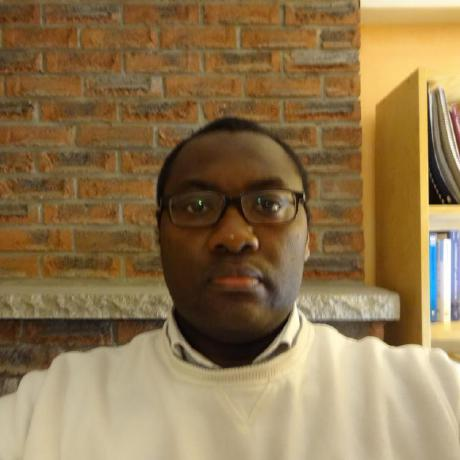
\includegraphics[scale=0.63]{images/XavierNOUNDOU-2}
\caption{Portrait de Xavier}~\label{fig:xaviernoumbis}
\end{figure}


\mainmatter

\chapter{Introduction}\label{chap:introduction}

\yeren est un syst\`eme logiciel de gestion des
stocks et de gestion des ventes. Il permet
d'ex\'ecuter des mouvements de stocks, et de
vendre des articles en stocks.

Une entreprise doit poss\'eder au minimum d'un stock
d'articles, d'un d\'ep\^ot ou d'une boutique pour utiliser
\yeren de fa\c{c}on efficace.\\

\begin{figure}[!htpb]
	\centering
	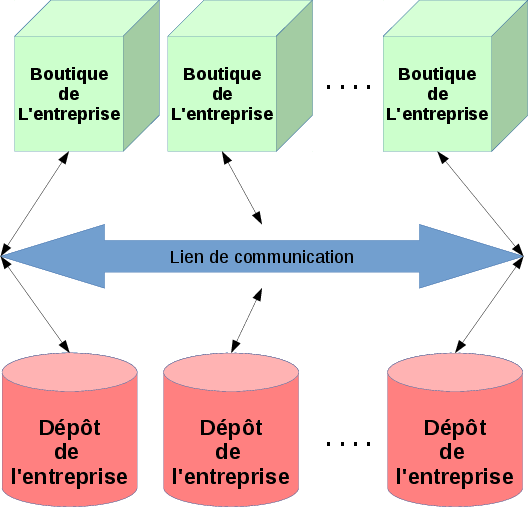
\includegraphics[scale=0.63]{images/architecture-enterprise-yeren.png}
	\caption{Un mod\`ele d'architecture d'une entreprise}\label{fig:architecture-enterprise-yeren}
\end{figure}

La figure~\ref{fig:architecture-enterprise-yeren} illustre
un mod\`ele g\'en\'erique d'entreprise o\`u les d\'ep\^ots
et les boutiques de l'entreprise sont en communication.

Les activit\'es principales de l'entreprise sont les suivantes:
\begin{enumerate}[1)]
	\item \emphbf{les sorties de stocks:} sortie d'articles
		d'une unit\'e (boutique ou d\'ep\^ot) pour r\'eception par un client
	\item \emphbf{les transferts de stocks:} mouvement d'articles
		d'une unit\'e vers une autre unit\'e
	\item \emphbf{les ventes d'articles:} un client ach\`ete
		des articles qui lui sont ensuite remis.\\
\end{enumerate}

\yeren permet d'accomplir les t\^aches de gestion
des stocks et de gestion des ventes suivantes:
\begin{enumerate}[1)]
	\item \myenumitem{cr\'eer des alertes sur des p\'eriodes de temps}	
	\item \myenumitem{cr\'eer des alertes sur des quantit\'e en stocks}	
	\item \myenumitem{entrer un stock}
	\item \myenumitem{lister les stocks}
	\item \myenumitem{modifier un stock}
	\item \myenumitem{supprimer un stock}	
	\item \myenumitem{rechercher des articles ou des stocks}
	\item \myenumitem{transf\'erer des articles ou des stocks}	
	\item \myenumitem{vendre des articles}	
	\item \myenumitem{visualiser les \'etats de transactions d'articles
		(sorties ou transferts de stocks)}
	\item \myenumitem{acc\'eder aux tableaux de bords}
	\item \myenumitem{visualiser les \'etats de ventes d'articles}.\\
\end{enumerate}

\newpage

\section{Acc\`es au manuel de l'utilisateur}

La figure~\ref{fig:fenetre-principale-utilisateur-non-enregistre}
illustre la fen\^etre d'accueil de \yeren sans aucun utilisateur
enregistr\'e.\\

\begin{figure}[!htbp]
\centering
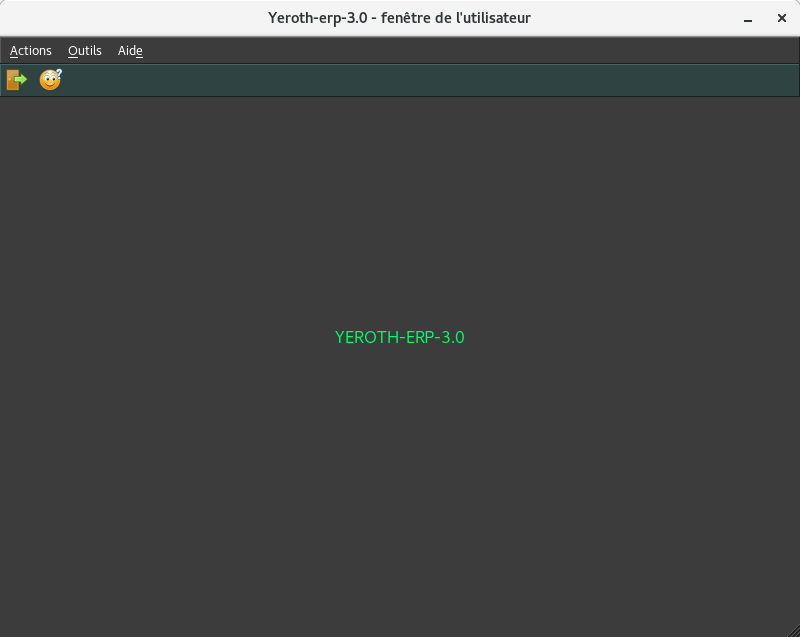
\includegraphics[scale=0.63]{images/yeren-fenetre-principale.png}
\caption{La fen\^etre d'acceuil sans aucun utilisateur enregistr\'e.}
\label{fig:fenetre-principale-utilisateur-non-enregistre}
\end{figure}

Il est requis qu'un utilisateur soit enregistr\'e
dans \yeren afin d'avoir acc\`es au manuel de l'utilisateur.

L'utilisateur de \yeren doit accomplir les op\'erations
suivantes afin d'avoir acc\`es au manuel de l'utilisateur:
\begin{enumerate}[1)]
	\item \`a partir de la fen\^etre d'accueil
		(voir figure~\ref{fig:fenetre-principale-utilisateur-non-enregistre}),
		cliquez sur le menu d\'eroulant '\textbf{Aide}'
	\item ensuite cliquez sur le lien '\textbf{Manuel de l'utilisateur (PDF)}'.
\end{enumerate}

\section{Structure de ce manuel de l'utilisateur}
Ce manuel de  l'utilisateur de \yeren est structur\'e
comme suit:

\begin{itemize}[\mycheckmark{purplish}]
	\item le chapitre~\ref{chap:utilisateurs} d\'ecrit
	les utilisateurs de \yeren et leurs \roles. 
	     
	\item le chapitre~\ref{chap:gestion-stocks} explicite
	les fonctionalit\'es de gestion des stocks

	\item le chapitre~\ref{chap:gestion-des-achats} parle
	de la gestion des achats
	
	\item le chapitre~\ref{chap:systeme-dalertes}
	pr\'esente le syst\`eme d'alertes sur les stocks
	
	\item le chapitre~\ref{chap:vendre} d\'ecrit comment
	conclure des ventes d'articles
	
	\item le chapitre~\ref{chap:sortir-articles} d\'ecrit
	comment proc\'eder \`a des sorties et transferts de stocks
	
	\item le chapitre~\ref{chap:vente} explicite comment
	rechercher et imprimer les \'etats de ventes d'articles
	
	\item le chapitre~\ref{chap:etats-des-sorties} explicite
	comment rechercher et imprimer les \'etats de sorties ou
	transferts d'articles
	
	\item le chapitre~\ref{chap:tableaux-de-bord} discute
	de la recherche et de la g\'en\'eration des rapports
	commerciaux de l'entreprise
	
	\item le chapitre~\ref{chap:informations-generales}
	explique comment avoir acc\`es aux d\'etails de
	l'utilisateur enregistr\'e, aux informations commerciales
	de l'entreprise, et enfin \`a la version de \yeren que
	l'on utilise
	
	\item le chapitre~\ref{chap:administration-logiciel}
	traite de l'administration du logiciel

	\item le chapitre~\ref{chap:problemes-connues}
	discute des probl\`emes connues de \yeren
	
	\item enfin, le chapitre~\ref{chap:conclusion} conclut
	ce manuel d'utilisation.
\end{itemize}


\nxsection{Le r\^ole ''Caissier''}\label{sec:utilisateurs-lecaissier}
\index{caissier}
\index{LeCaissier}

La figure~\ref{fig:fenetre-principale-caissier} illustre la
fen\^etre d'acceuil d'un utilisateur avec le \role \caissier,
apr\`es qu'il se soit enregistr\'e dans \yeren.\\

\begin{figure}[!htbp]
\centering
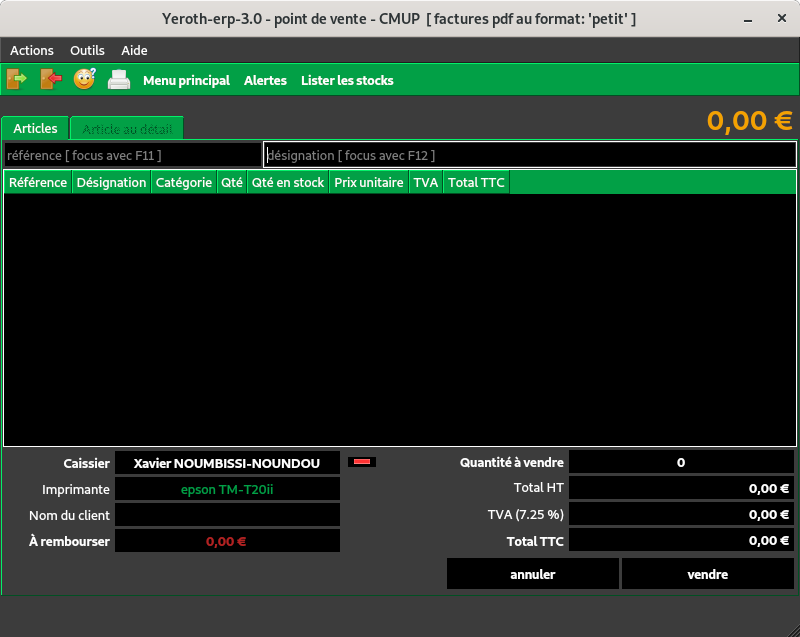
\includegraphics[scale=0.63]{images/yeren-fenetre-caissier.png}
\caption{La fen\^etre d'acceuil d'un caissier.}
\label{fig:fenetre-principale-caissier}
\end{figure}

Un utilisateur de \yeren avec le \role "\caissier" assume
les t\^aches suivantes:
\begin{enumerate}[1)]
	\item lister les stocks \`a partir de l'interface de vente	
	\item visualiser une facture proforma		
	\item imprimer une facture proforma
	\item vendre un ou plusieurs stocks (ou articles).\\
\end{enumerate}
\chapter{Point De Vente (La Vente d'Articles)}\label{chap:vendre}
\index{vendre des articles}
\index{vendre des stocks}

\utilisateurs: \liencaissier, \lienmanager.\\

\chapintro{Ce chapitre d\'ecrit comment vendre des articles,
appliquer des rabais, et appliquer la TVA sur un
article ou la retirer.}

\nxsection{Introduction}\label{sec:vendre-introduction}

La figure~\ref{fig:fenetre-vendre} illustre
l'interface graphique pour proc\'eder \`a la
vente d'articles.

\begin{figure}[!htbp]
	\centering
	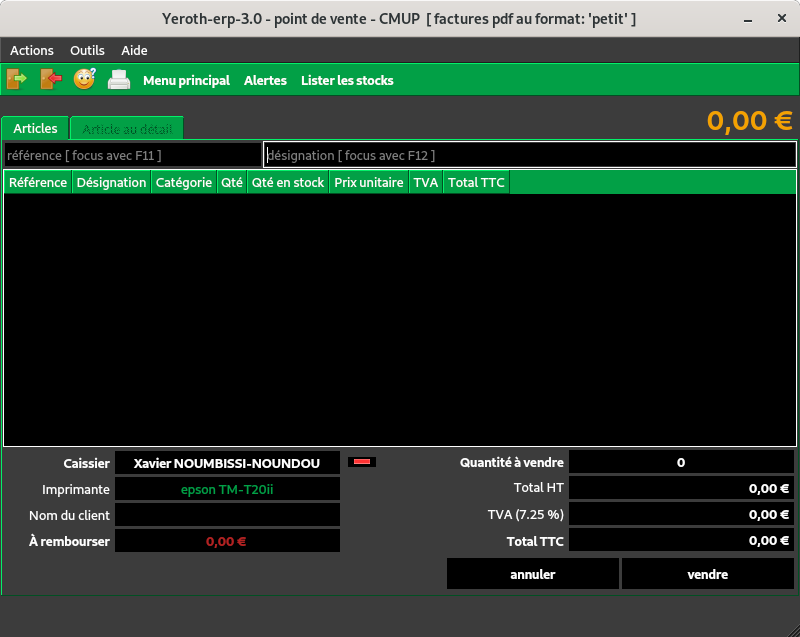
\includegraphics[scale=0.63]{images/yeren-fenetre-caissier.png}
	\caption{La fen\^etre pour vendre les articles.}
	\label{fig:fenetre-vendre}
\end{figure}

Le tableau o\`u sont affich\'es les articles \`a vendre
a les colones suivantes:
\begin{enumerate}[1)]
	\item R\'ef\'erence
	\item D\'esignation
	\item P.U. (\textbf{Prix Unitaire})
	\item Qt\'e (\textbf{Quantit\'e})
	\item Qt\'e restante en stock (\textbf{Quantit\'e restante en stock})
	\item Total TTC (\textbf{Total Toute Taxes Comprise})	
	\item TVA (\textbf{Taxe sur la Valeur Ajout\'e}).
\end{enumerate}

\subsection{La strat\'egie de vente utilis\'ee}
\index{La strat\'egie de vente des articles}
\index{La strat\'egie de vente des stocks}

Le titre de la fen\^etre affiche la strat\'egie de vente
des stocks utilis\'ee. Dans la figure~\ref{fig:fenetre-vendre}
par exemple, la strat\'egie de vente utilis\'ee est
\cmup.

\newpage
%-----------------------------------------------------------

\nxsection{S\'electionner des articles
	\`a vendre}\label{sec:selectionner-articles-vendre}
\index{s\'electionner des articles \`a vendre}
\index{s\'electionner des stocks \`a vendre}

Il existe $2$ m\'ethodes pour s\'electionner des articles
\`a vendre:
\begin{itemize}[\mycheckmark{purplish}]
	\item \textcolor{purplish}{$\mathbf{1^{\text{\`ere}}}$ \textbf{m\'ethode}}\\
	S\'electionner les stocks des articles \`a vendre
	en entrant leur code bar dans le premier champs de texte
	de l'interface (voir figure~\ref{fig:yeren-vendre-choisir-stock-codebar})
	\begin{figure}[!htbp]
		\centering
		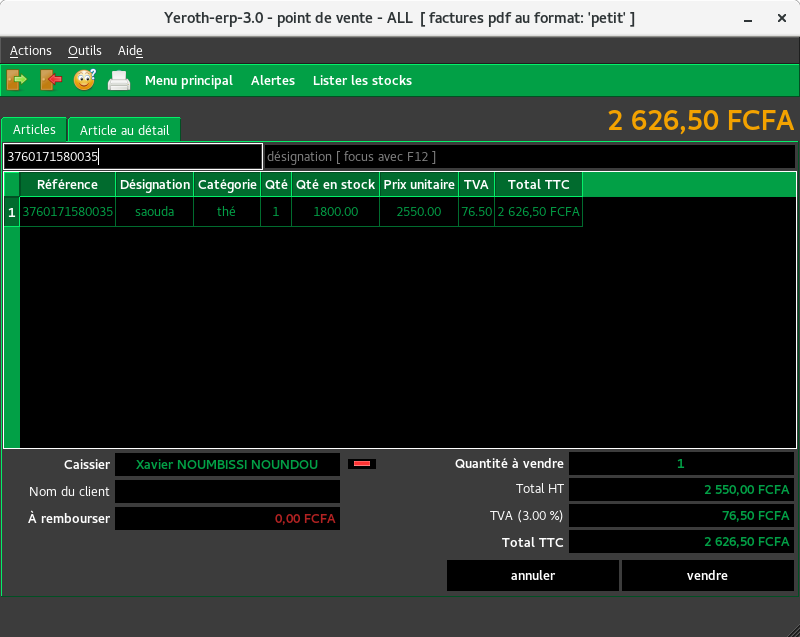
\includegraphics[scale=0.63]{images/yeren-vendre-choisir-stock-codebar.png}
		\caption{Le champs de texte pour
			ajouter les articles en utilisant leur code bar.}\label{fig:yeren-vendre-choisir-stock-codebar}
	\end{figure}
	
	\newpage
	\item \textcolor{purplish}{$\mathbf{2^{\text{\`eme}}}$ \textbf{m\'ethode}}\\
	S\'electionner les stocks des articles \`a vendre
	en entrant leur d\'esignation dans le deuxi\`eme
	champs de texte de l'interface
	(voir figure~\ref{fig:yeren-vendre-choisir-stock-designation}).
	\begin{figure}[!htbp]
		\centering
		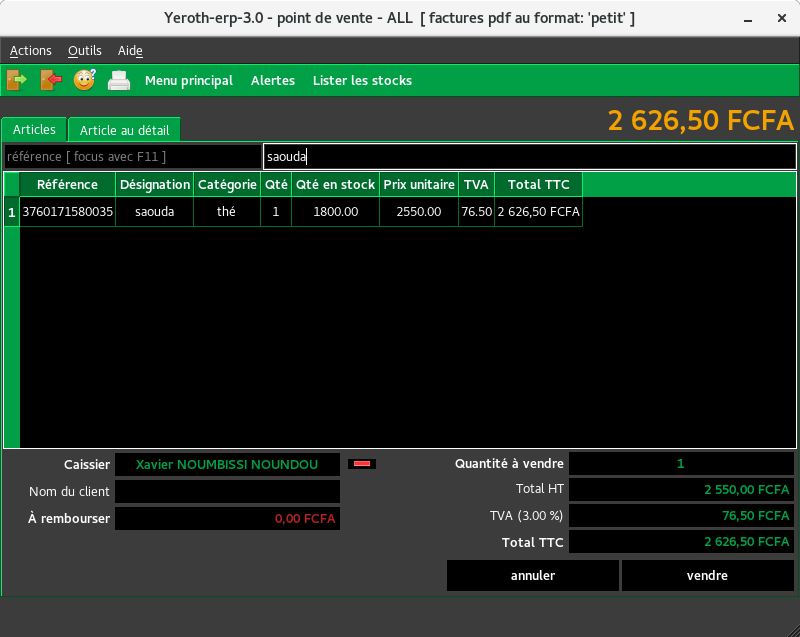
\includegraphics[scale=0.63]{images/yeren-vendre-choisir-stock-designation.png}
		\caption{Le champs de texte pour
			ajouter les articles en utilisant leur d\'esignation.}\label{fig:yeren-vendre-choisir-stock-designation}
	\end{figure}
\end{itemize}

\newpage

%----------------------------------------------------------- 

\nxsection{Afficher les d\'etails d'un article / stock
			s\'electionn\'e pour la vente}
\index{afficher les d\'etails d'un article \`a vendre}
\index{afficher les d\'etails d'un stock \`a vendre}

La figure~\ref{fig:yeren-vente-afficher-details-stock}
illustre les d\'etails du stock 'Saouda'.

Il existe deux m\'etodes pour voir les d\'etails
d'un stock s\'electionn\'e pour la vente:
\begin{itemize}[\mycheckmark{purplish}]
	\item \textcolor{purplish}{$\mathbf{1^{\text{\`ere}}}$ \textbf{m\'ethode}}\\
	Il suffit de cliquer deux fois sur n'importe quelle
	partie autre que '\textbf{Qt\'e}' de la ligne du
	stock s\'electionn\'e.\\
	
	\item \textcolor{purplish}{$\mathbf{2^{\text{\`eme}}}$ \textbf{m\'ethode}}\\
	Il suffit de cliquer sur l'onglet '\textbf{Article au d\'etail}'
	apr\`es la s\'election du stock.
\end{itemize}

%-----------------------------------------------------------
\newpage
\nxsection{Changer la quantit\'e \`a vendre
			d'un article / stock}\label{sec:changer-qte-vendre}
\index{changer la quantit\'e d'un article \`a vendre}
\index{changer la quantit\'e d'un stock \`a vendre}

Il existe deux m\'etodes pour changer la quantit\'e
d'articles d'un stock:
\begin{itemize}[\mycheckmark{purplish}]
	\item \textcolor{purplish}{$\mathbf{1^{\text{\`ere}}}$ \textbf{m\'ethode}}\\
	il faut cliquer sur l'\'el\'ement '\textbf{Qt\'e}'
	avec le bouton gauche de la souris, et ensuite changer la
	quantit\'e \`a vendre (voir figure~\ref{fig:yeren-vendre-qte-selectionner})
	\begin{figure}[!htbp]
		\centering
		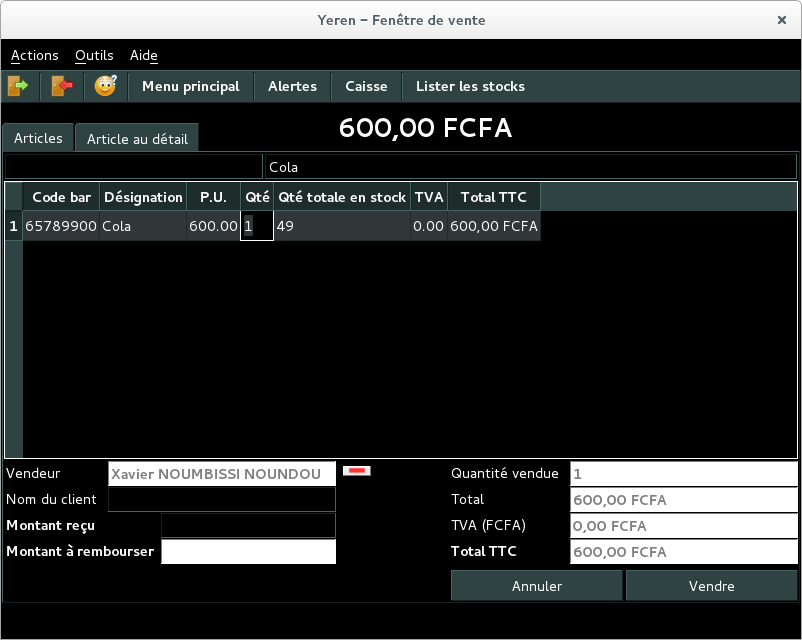
\includegraphics[scale=0.63]{images/yeren-vendre-qte-selectionner.png}
		\caption{L'\'el\'ement 'Qt\'e' s\'electionn\'e pour
			changer la quantit\'e d'articles 'Cola' \`a vendre.}\label{fig:yeren-vendre-qte-selectionner}
	\end{figure}
	\newpage
	
	\item \textcolor{purplish}{$\mathbf{2^{\text{\`eme}}}$ \textbf{m\'ethode}}\\
	il faut cliquer deux fois sur n'importe quel autre
	partie de la ligne du stock s\'electionn\'e, autre que 'Qt\'e'
	pour avoir acc\`es \`a une vue d\'etaill\'ee de ce stock.\\
	
	La vue de d\'etails du stock permet de changer
	la quantit\'e \`a vendre dans le champ de texte
	'\textbf{quantit\'e \`a vendre}'
	(voir figure~\ref{fig:yeren-vente-afficher-details-stock}).
	\begin{figure}[!htbp]
		\centering
		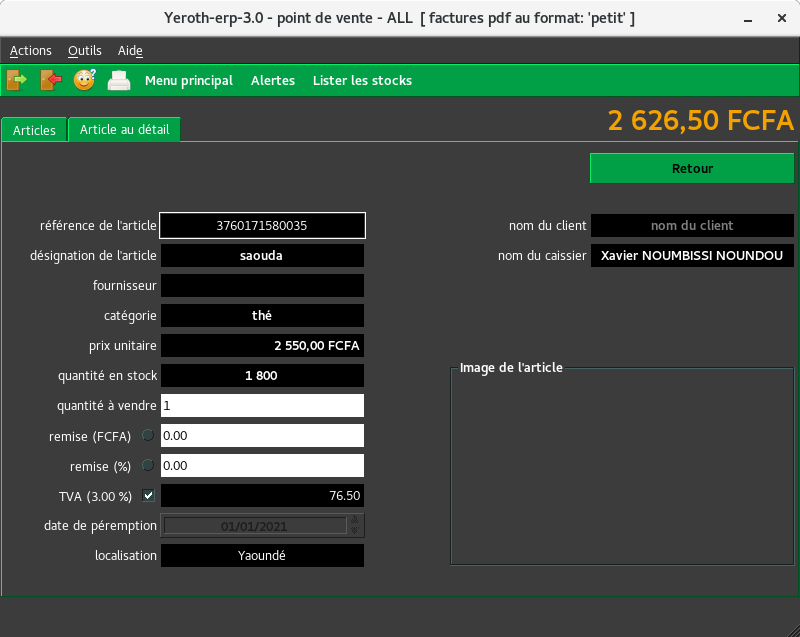
\includegraphics[scale=0.63]{images/yeren-vente-afficher-details-stock.png}
		\caption{Le champs de texte 'quantit\'e \`a vendre'
			permet de changer la quantit\'e \`a vendre d'un article.}
			\label{fig:yeren-vente-afficher-details-stock}
	\end{figure}
\end{itemize}

%-----------------------------------------------------------

\newpage
\nxsection{Appliquer une remise sur
			un article / stock \`a vendre}\label{sec:appliquer-remise-sur-article}
\index{appliquer un rabais sur un article}
\index{appliquer une remise sur un article}
\index{appliquer un rabais sur un stock}
\index{appliquer une remise sur un stock}

Voici la d\'emarche \`a suivre pour appliquer une remise
sur le prix unitaire d'un article \`a vendre:

\begin{enumerate}[1)]
	\item S\'electionner l'article \`a vendre (voir section~\ref{sec:selectionner-articles-vendre})
	\item ouvrer la vue de d\'etails de l'article auquel
		vous souhaitez appliquer une remise
		
	\item appliquer la remise en FCFA ou en pourcentage,
		en choisissant respectivement les bouton de radio
		\bouton{remise (FCFA)} ou \bouton{remise (\%)}, et
		en entrant le montant ou le pourcentage de remise
		\`a appliquer. (voir figure~\ref{fig:yeren-vente-afficher-details-stock})
		
	\item vous pouvez ensuite conclure la vente (voir section~\ref{sec:conclure-une-vente}).
\end{enumerate} 

%-----------------------------------------------------------

\nxsection{Modifier la TVA sur un article \`a vendre}\label{sec:modifier-TVA-article}
\index{ajouter la TVA sur le co\^ut d'un article}
\index{supprimer la TVA sur co\^ut d'un article}

Voici la d\'emarche \`a suivre pour retirer ou ajouter
la TVA sur un article \`a vendre:

\begin{enumerate}[1)]
	\item S\'electionner l'article \`a vendre (voir section~\ref{sec:selectionner-articles-vendre})
	\item ouvrer la vue de d\'etails de l'article auquel
	vous souhaitez appliquer une remise
	
	\item retirer ou ajouter la TVA en cochant le 'check box'
	TVA (voir figure~\ref{fig:yeren-vente-afficher-details-stock}).
	
	\item vous pouvez ensuite conclure la vente (voir section~\ref{sec:conclure-une-vente}).
\end{enumerate} 

%-----------------------------------------------------------
\newpage
\nxsection{Supprimer un article de la liste des articles \`a vendre}
\index{supprimer un article de la liste des articles \`a vendre}

\begin{figure}[!htbp]
	\centering
	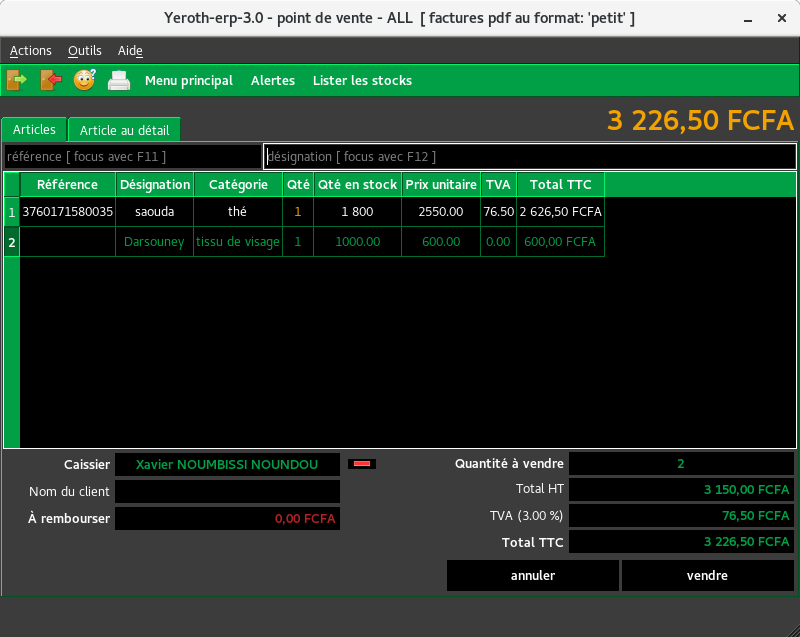
\includegraphics[scale=0.63]{images/yeren-vendre-supprimer-article.png}
	\caption{Le bouton rouge sert \`a supprimer un article
		de la liste des articles \`a vendre.}
	\label{fig:yeren-vendre-supprimer-article}
\end{figure}

Il suffit de s\'electionner la ligne de l'article \`a vendre,
et ensuite cliquer sur le petit bouton rouge qui se trouve
juste apr\`es le champs de texte '\textbf{Caissier}'.

Ce bouton rouge est illustr\'e dans la figure~\ref{fig:yeren-vendre-supprimer-article},
juste apr\`es le champs de texte '\textbf{Caissier}'.
	
%-----------------------------------------------------------
\newpage
\nxsection{Vendre \`a un client divers}\label{sec:vendre-client-divers}
\index{vendre \`a un client divers}

Il suffit de laisser le champs de texte '\textbf{Nom du client}'
vide lors de la vente.

%-----------------------------------------------------------

\nxsection{Vendre \`a un client nomm\'e}\label{sec:vendre-client-nomme}
\index{vendre \`a un client nomm\'e}

Il suffit de saisir le nom du client dans le champs de
texte '\textbf{Nom du client}'.

\begin{figure}[!htbp]
	\centering
	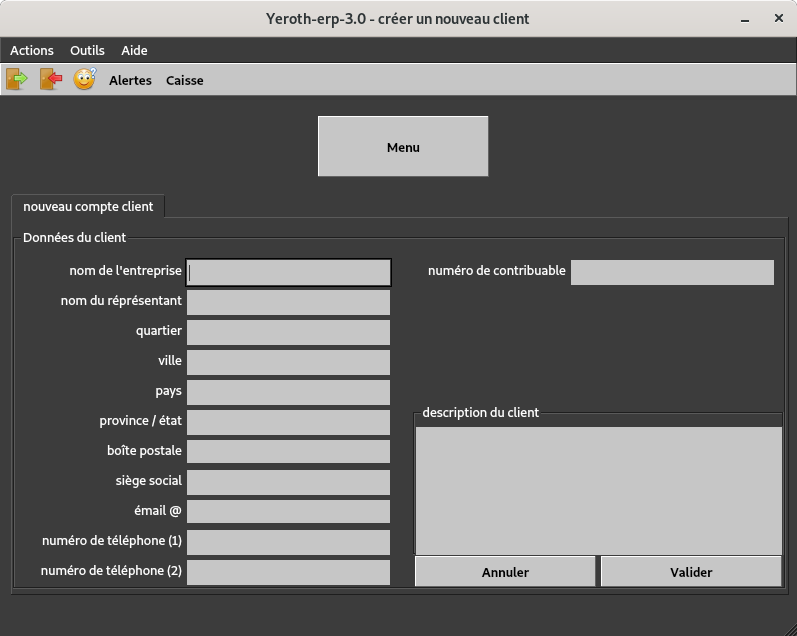
\includegraphics[scale=0.63]{images/yeren-vente-creer-nouveau-client.png}
	\caption{La fen\^etre de la cr\'eation d'un nouveau compte
		client \`a partir de l'interface de vente.}
	\label{fig:yeren-vente-creer-nouveau-client}
\end{figure}

Si le nom du client n'appara\^it pas dans la liste
sugg\'er\'ee, l'utilisateur doit s\'electionner le texte
'\textbf{nouveau client (*)}' (dans la liste sugg\'er'ee).
L'utilisateur sera alors conduit \`a la fen\^etre
pour cr\'eer un nouveau compte client
(figure~\ref{fig:yeren-vente-creer-nouveau-client}).

%-----------------------------------------------------------

\nxsection{Annuler une vente en cours}
\index{annuler une vente en cours}

Il suffit de cliquer sur le bouton \bouton{Annuler} pour annuler
une vente en cours.

%-----------------------------------------------------------

\nxsection{Conclure une vente}\label{sec:conclure-une-vente}
\index{conclure une vente}

Voici la d\'emarche \`a suivre pour conclure une vente:

\begin{enumerate}[1)]
	\item s\'electionner les articles \`a vendre
	(voir section~\ref{sec:selectionner-articles-vendre})
	
	\item entrer les quantit\'es \`a vendre 
	(voir section~\ref{sec:changer-qte-vendre})
	
	\item s'il y'a lieu, appliquer des remises ou modifier
	la TVA (voir section~\ref{sec:appliquer-remise-sur-article})
	
	\item enfin, retourner \`a la fen\^etre titr\'ee
	'\textbf{Yeroth-erp-3.0 - Fen\^etre de la vente'} et
	presser sur le bouton \bouton{Vendre}
	(voir figure~\ref{fig:yeren-vendre-supprimer-article}).
\end{enumerate}

%-----------------------------------------------------------
\nxsection{Imprimer la facture \`a la suite d'une vente}
\index{imprimer la facture \`a la suite d'une vente}
\index{un exemple de facture}

\begin{figure}[!htbp]
	\centering
	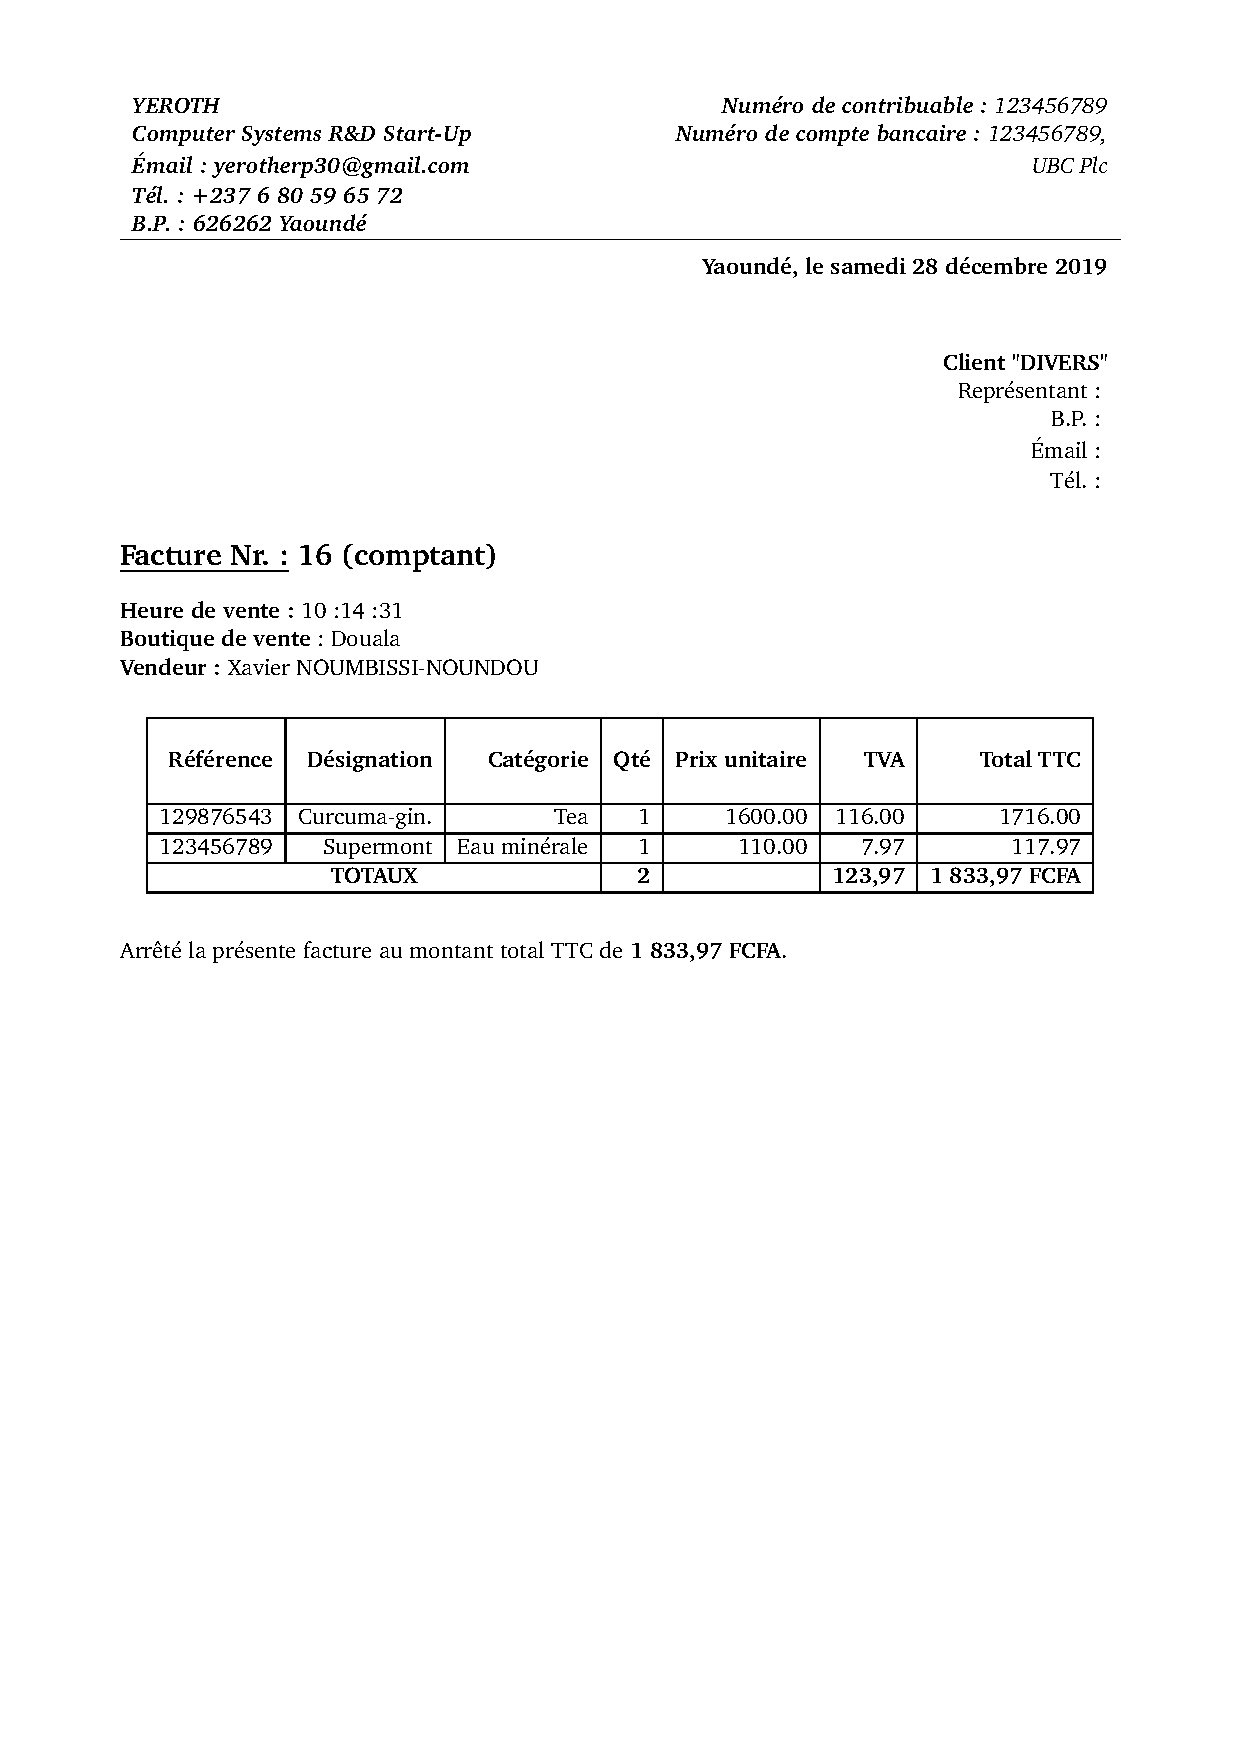
\includegraphics[scale=0.75]{images/yeren-facture-grand-2017-06-13.pdf}
	\caption{Une facture g\'en\'er\'ee \`a la suite d'une vente.}
	\label{fig:yeren-vendre-facture}
\end{figure}

Une facture au format PDF est automatiquement
g\'en\'erer, juste apr\`es qu'une vente soit effectu\'ee.
La figure~\ref{fig:yeren-vendre-facture} illustre un
exemple de facture.

%----------------------------------------------------------- 

\nxsection{Imprimer un exemple de facture au format
	PDF avant de conclure une vente}
\index{un exemple de facture au format PDF}
\index{imprimer un exemple de facture au format PDF}

\begin{figure}[!htbp]
	\centering
	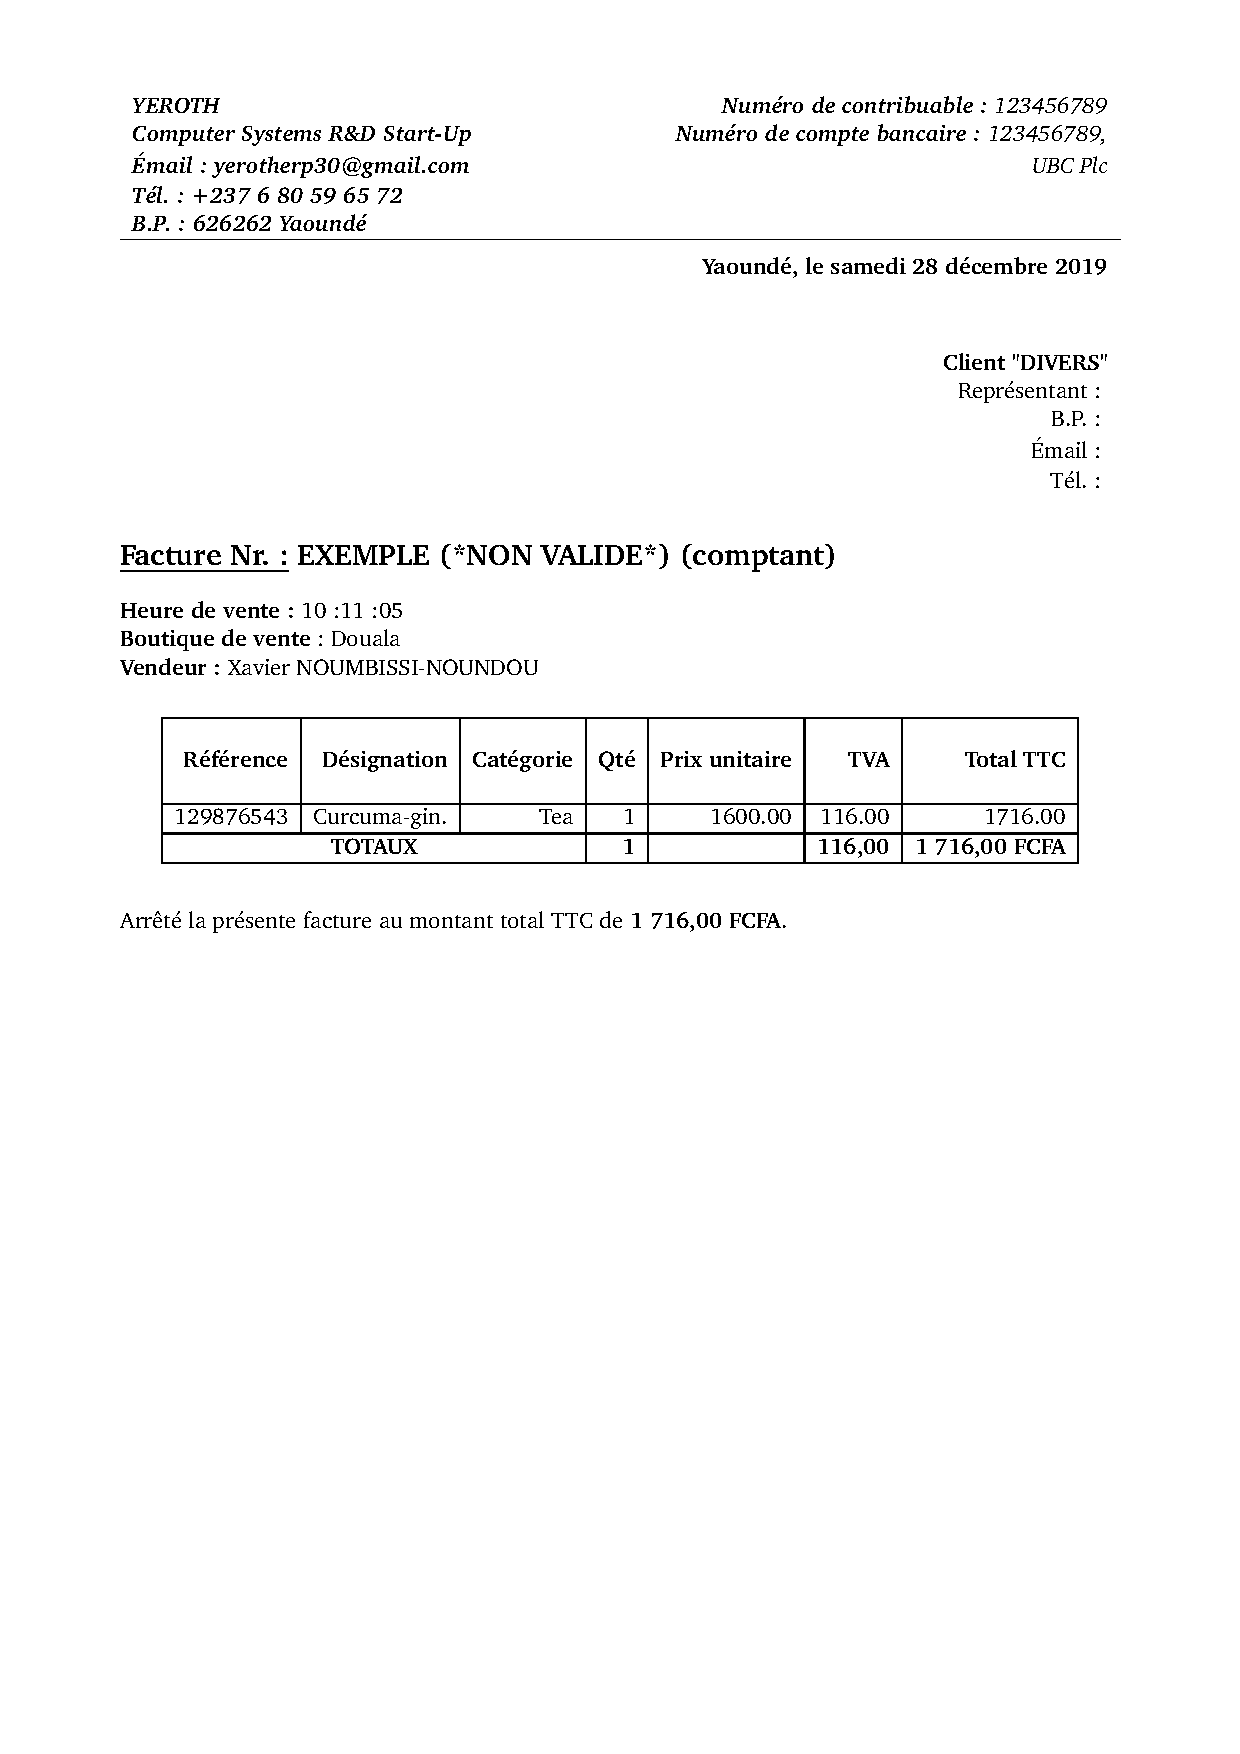
\includegraphics[scale=0.75]{images/yeren-exemple-facture-grand-2017-06-13.pdf}
	\caption{Une facture proforma g\'en\'er\'ee avant de conclure une vente.}
	\label{fig:yeren-vendre-facture-proforma}
\end{figure}

Il existe deux m\'ethodes pour imprimer une facture
proforma avant de conclure la vente \'eventuelle des articles
pr\'esents dans le tableau qui appara\^it dans la fen\^etre
titr\'ee '\textbf{Yeroth-erp-3.0 - Fen\^etre de la vente}'.

\begin{itemize}[\mycheckmark{purplish}]
	\item \textcolor{purplish}{$\mathbf{1^{\text{\`ere}}}$ \textbf{m\'ethode}}\\
		Cliquer sur le lien '\textbf{Imprimer la facture (proforma)}'
		qui se trouve dans le menu d\'eroulant '\textbf{Outils}'\\

	\item \textcolor{purplish}{$\mathbf{2^{\text{\`eme}}}$ \textbf{m\'ethode}}\\
		Presser simultan\'ement les boutons \bouton{CTRL}
		et \bouton{P} de votre clavier.
\end{itemize}

Une facture proforma au format PDF est alors g\'en\'er\'ee. Un
exemple de facture proforma est illustr\'e dans la
figure~\ref{fig:yeren-vendre-facture-proforma}.

\chapter{Les Ventes (les \'etats des ventes d'articles)}\label{chap:vente}
\index{vente}
\index{\'etats des ventes d'articles}
\index{\'etats des ventes des stocks}

\utilisateurs: \liencaissier, \lienmanager.\\

\chapintro{Ce chapitre d\'ecrit comment consulter
les chiffres d'affaires (les recettes). Le chapitre
explique aussi comment param\'etrer cette
consultation afin d'obtenir des r\'esultats
plus pr\'ecis (ex: le chiffre d'affaire r\'ealis\'e
sur un article).}

\nxsection{Introduction}

\begin{figure}[!htpb]
	\centering
	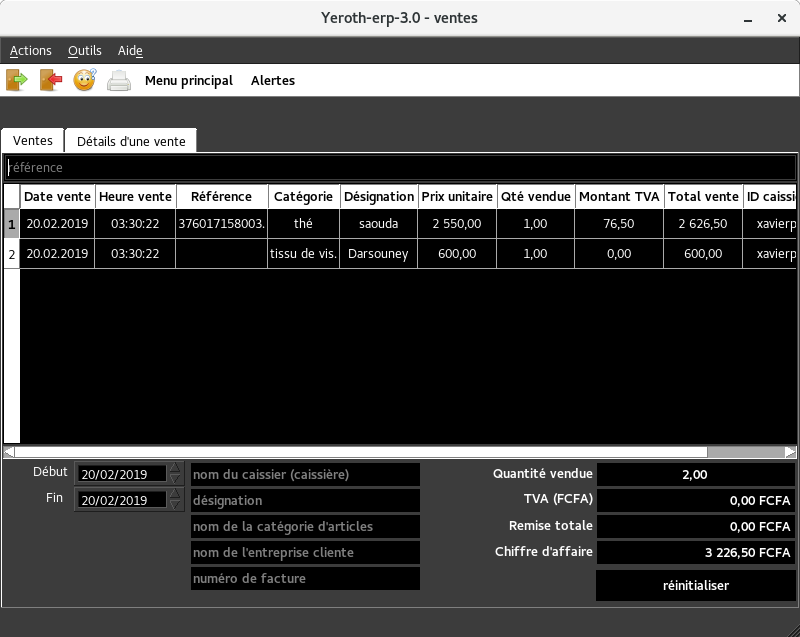
\includegraphics[scale=0.63]{images/yeren-caisse.png}
	\caption{La fen\^etre du module caisse
				(les \'etats de ventes)}~\label{fig:yeren-caisse}
\end{figure}

Le module '\textbf{Caisse}' de \yeroth donne une
vue d'ensemble sur toutes les ventes effectu\'ees.
La figure~\ref{fig:yeren-caisse} illustre
l'interface graphique du module '\textbf{Caisse}'.

%-----------------------------------------------------------

\nxsection{Voir le journal des ventes sur une p\'eriode de temps}
\index{consulter le journal des ventes}
\index{voir le journal des ventes}
\index{historique des ventes}

Un utilisateur \textbf{avec le \role \manager} d\'efinit
les dates de d\'ebut et de fin de la p\'eriode sur
laquelle il souhaite voir les ventes. Il peut aussi
ajouter les param\`etres suivants \`a sa requ\^ete:

\begin{enumerate}[1)]
	\item le nom d'un caissier 
		(champs de texte '\textbf{Caissier}')
	\item la d\'esignation d'un l'article
		(champs de texte '\textbf{D\'esignation}')
	\item une cat\'egorie d'articles
		(champs de texte '\textbf{Cat\'egorie}')
	\item le nom d'un client
		(champs de texte '\textbf{Client}')
	\item le num\'ero d'une facture.
		(champs de texte '\textbf{Facture N.}').
\end{enumerate}

Lorsque plus d'un param\`etre est utilis\'e pour la requ\^ete,
\yeroth emploi l'op\'erateur logique '\textbf{AND}' pour
g\'en\'erer la requ\^ete.

\textbf{NB:} les utilisateurs \textbf{avec le \role \caissier}
ont seulement acc\`es \`a leur journal des ventes du jour.
Ils ont aussi acc\`es au param\'etrage des \'el\'ements
suivants:

\begin{enumerate}[1)]
	\item la d\'esignation d'un l'article
		(champs de texte '\textbf{D\'esignation}')
	\item une cat\'egorie d'articles
		(champs de texte '\textbf{Cat\'egorie}')
	\item le num\'ero d'une facture.
		(champs de texte '\textbf{Facture N.}').
\end{enumerate}

%-----------------------------------------------------------

\nxsection{Voir les d\'etails d'une vente}
\index{consulter les d\'etails d'une vente}
\index{voir les d\'etails d'une vente}

Il suffit de cliquer deux fois sur la vente s\'electionn\'ee.

%-----------------------------------------------------------

\nxsection{Voir le journal des ventes d'un caissier}
\index{voir le journal des ventes d'un caissier}
\index{voir le chiffre d'affaire r\'ealis\'e avec un caissier}
\index{chiffre d'affaire d'un caissier}

Il suffit de param\'etrer la requ\^ete avec le nom de ce
caissier dans le champs de texte '\textbf{Caissier}' (Voir
la figure~\ref{fig:yeren-caisse}).

%-----------------------------------------------------------

\nxsection{Voir le journal des ventes d'un article}
\index{voir le journal des ventes d'un article}
\index{voir le chiffre d'affaire r\'ealis\'e avec un article}
\index{chiffre d'affaire d'un article}

Il suffit de param\'etrer la requ\^ete avec la d\'esignation
de cet article. Ceci se fait dans le champs de texte
'\textbf{D\'esignation}' (Voir la figure~\ref{fig:yeren-caisse}).

%-----------------------------------------------------------

\nxsection{Voir le journal des ventes d'une cat\'egorie d'articles}
\index{voir le journal des ventes d'une cat\'egorie d'articles}
\index{voir le journal des ventes d'une famille d'articles}
\index{voir le chiffre d'affaire r\'ealis\'e avec une famille d'articles}
\index{chiffre d'affaire d'une cat\'egorie d'articles}

Il suffit de param\'etrer la requ\^ete avec le nom de la
cat\'egorie de cet article. Ceci se fait dans le champs
de texte '\textbf{Cat\'egorie}' (Voir la figure~\ref{fig:yeren-caisse}).

%-----------------------------------------------------------

\nxsection{Voir le journal des achats d'un client nomm\'e}
\index{voir le journal des achats d'un client nomm\'e}
\index{voir le chiffre d'affaire r\'ealis\'e avec un client nomm\'e}

Il suffit de param\'etrer la requ\^ete avec le nom du
client concern\'e. Ceci se fait dans le champs de
texte '\textbf{Client}' (Voir la figure~\ref{fig:yeren-caisse}).

%-----------------------------------------------------------

\nxsection{Voir le journal des ventes d'une facture}
\index{voir les ventes d'une facture}

Il suffit de param\'etrer la requ\^ete avec le num\'ero
de facture correspondant. Ceci se fait dans le champs de
texte '\textbf{Facture N.}' (Voir la figure~\ref{fig:yeren-caisse}).

%-----------------------------------------------------------

\nxsection{Imprimer le journal des ventes au format PDF}
\index{Imprimer le journal des ventes au format PDF}

Il existe deux m\'ethodes pour imprimer 'le journal
des ventes' de la liste des ventes qui appara\^it \`a
la fen\^etre titr\'e '\textbf{Yeroth-erp-3.0 - Caisse}'.

\begin{itemize}[\mycheckmark{purplish}]
	\item \textcolor{purplish}{$\mathbf{1^{\text{\`ere}}}$ \textbf{m\'ethode}}\\
		Cliquer sur le lien '\textbf{Imprimer le journal des
		ventes}' qui se trouve dans le menu
		d\'eroulant '\textbf{Outils}'\\

	\item \textcolor{purplish}{$\mathbf{2^{\text{\`eme}}}$ \textbf{m\'ethode}}\\
		Presser simultan\'ement les boutons \bouton{CTRL}
		et \bouton{P} de votre clavier.
\end{itemize}

\chapter{Les Informations G\'en\'erales}\label{chap:informations-generales}

\utilisateurs: \lienadmin, \liencaissier, \lienmagasinier, \lienmanager.\\

\chapintro{Ce chapitre d\'ecrit comment avoir acc\`es aux
informations publiques de l'entreprise et de \yeroth
(ex.: le si\`ege social de l'entreprise, la version
de \yeroth utilis\'ee, etc).}

\nxsection{Voir les d\'etails de l'utilisateur avec lequel
			on s'est enregistr\'e}
\index{voir les d\'etails de l'utilisateur avec lequel
		on s'est enregistr\'e}

\begin{figure}[!htbp]
	\centering
	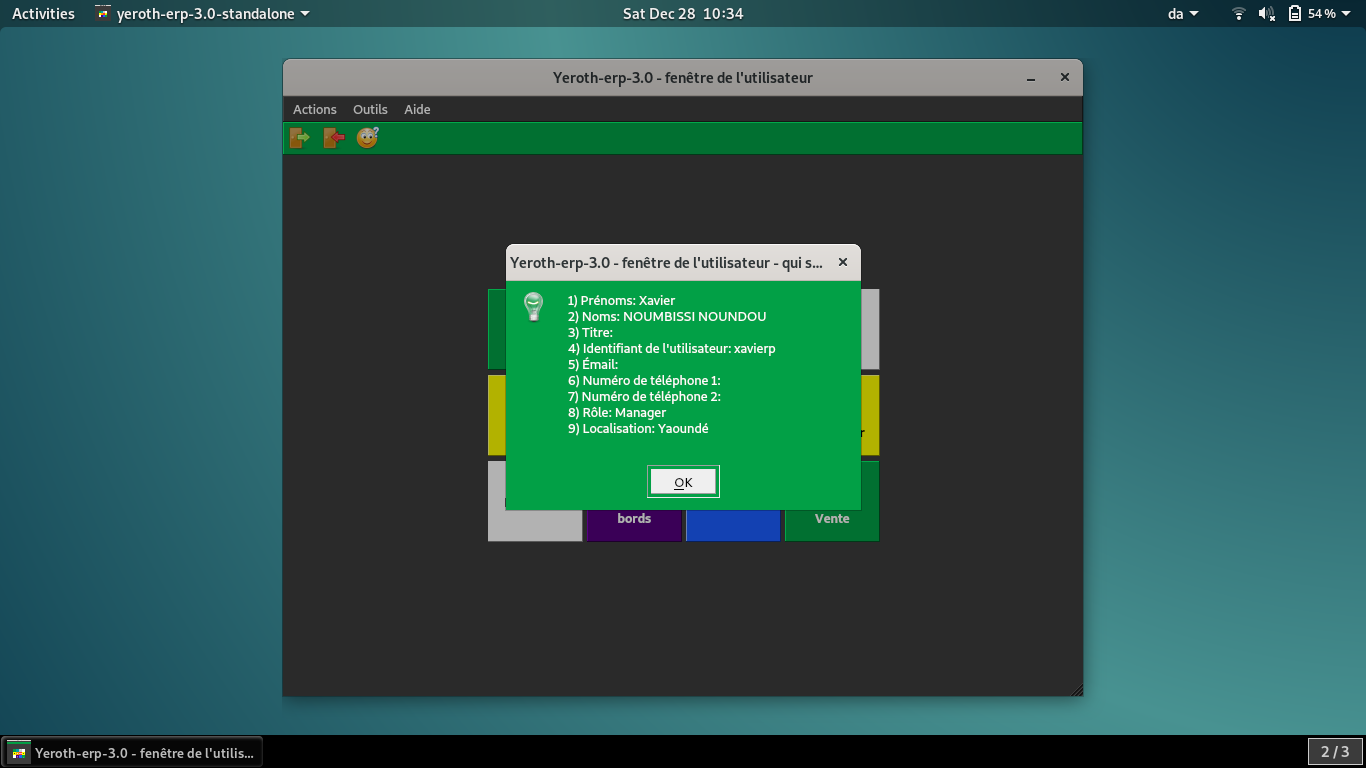
\includegraphics[scale=0.34]{images/yeren-qui-suis-je.png}
	\caption{Un example de la fonctionalit\'e 'Qui suis je ?'.}
	\label{fig:yeren-qui-suis-je}
\end{figure}

La figure~\ref{fig:yeren-qui-suis-je} illustre un example de
la fonctionalit\'e '\textbf{Qui suis je ?}'.

\`A partir de n'importe quelle fen\^etre de \yeroth, cliquez
sur le lien '\textbf{Qui suis je ?}' dans le menu d\'eroulant
'\textbf{Outils}' pour obtenir les informations suivantes
de l'utilisateur avec lequel on s'est enregistr\'e:

\begin{enumerate}[1)]
	\item l'\'email
	\item l'identification de l'utilisateur	
	\item la localisation
	\item les noms	
	\item le num\'ero de t\'el\'ephone 1
	\item le num\'ero de t\'el\'ephone 2	
	\item les pr\'enoms
	\item le r\^ole	
	\item le titre.
\end{enumerate}

%---------------------------------------------------------------

\nxsection{Voir les informations g\'en\'erales de l'entreprise}
\index{voir les informations g\'en\'erales de l'entreprise}

\`A partir de n'importe quelle fen\^etre de \yeroth (except\'e
les fen\^etres de l'administration), cliquez
sur le lien '\textbf{Informations sur l'entreprise}' dans
le menu d\'eroulant '\textbf{Aide}' pour obtenir les
informations suivantes de l'entreprise o\`u \yeroth
est ainsi d\'eploy\'e:

\begin{enumerate}[1)]
	\item l'\'email
	\item l'adresse
	\item la bo\^ite postale
	\item la d\'enomination de l'entreprise
	\item la localisation
	\item le num\'ero de contribuable	
	\item le pays
	\item les secteurs d'activit\'es
	\item le si\`ege social
	\item le t\'el\'ephone
	\item la ville.
\end{enumerate}

La figure~\ref{fig:yeren-informations-generales-entreprise}
illustre un example de la fonctionalit\'e 
'\textbf{Informations sur l'entreprise}'.\\

\begin{figure}[!htbp]
	\centering
	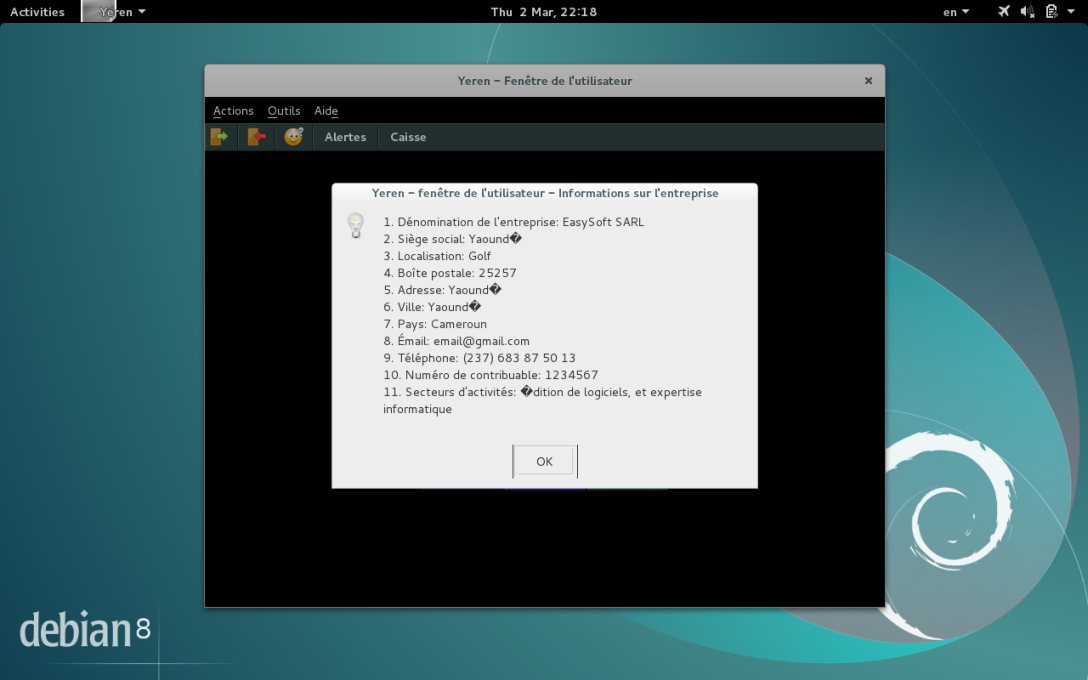
\includegraphics[scale=0.4]{images/yeren-informations-generales-entreprise.png}
	\caption{Un example de la fonctionalit\'e 'Informations sur l'entreprise'.}
	\label{fig:yeren-informations-generales-entreprise}
\end{figure}

%---------------------------------------------------------------

\newpage
\nxsection{Voir le manuel de l'utilisateur au format PDF}
\index{manuel de l'utilisateur au format PDF}

Il suffit de cliquer sur le lien '\textbf{Manuel de l'utilisateur (PDF)}'
qui se trouve dans le menu '\textbf{Aide}' de la fen\^etre
principale de chaque type d'utilisateur de \yeroth:

\begin{enumerate}[1)]
	\item \admin (voir figure~\ref{fig:fenetre-principale-admin})
	\item \caissier (voir figure~\ref{fig:fenetre-principale-caissier})
	\item \magasinier (voir figure~\ref{fig:yeren-fenetre-magasinier})
	\item \manager (voir figure~\ref{fig:yeren-fenetre-patron}).		
\end{enumerate}

%---------------------------------------------------------------

\nxsection{Voir la version de \yeroth que vous utilis\'e}
\index{voir la version de \yeroth que vous utilis\'e}

Il suffit de cliquer sur le lien '\textbf{\`A propos}' qui
se trouve dans le menu '\textbf{Aide}' de n'importe quelle
fen\^etre de \yeroth.

La figure~\ref{fig:yeren-apropos}
illustre un example de la fonctionalit\'e 
'\textbf{\`A propos}'.

\begin{figure}[!htbp]
	\centering
	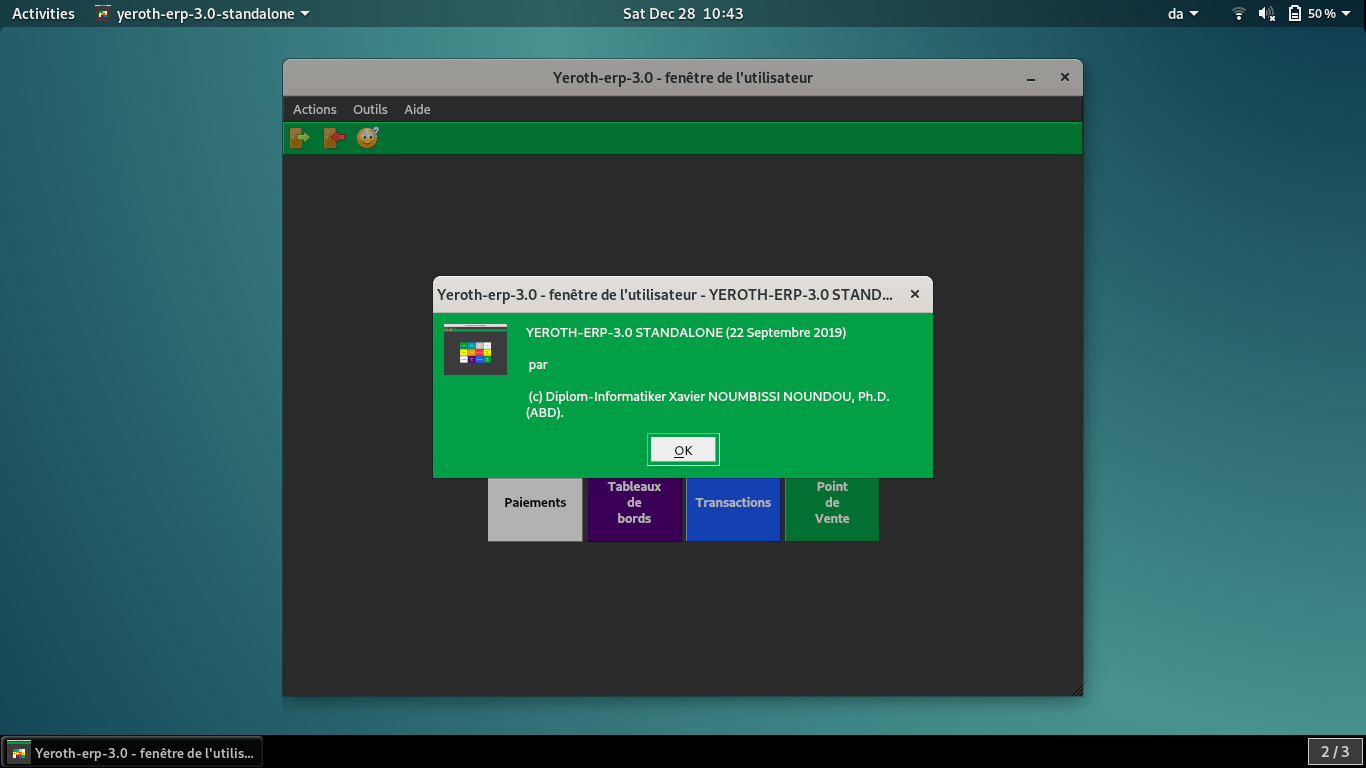
\includegraphics[scale=0.369]{images/yeren-apropos.png}
	\caption{Un example de la fonctionalit\'e '\`A propos'.}
	\label{fig:yeren-apropos}
\end{figure}



\chapter{Les Probl\`emes Connues et leurs Solutions}\label{chap:problemes-connues}
\index{probl\`emes connues ! solutions}
\index{probl\`emes connues et solutions}

\chapintro{Ce chapitre d\'ecrit quelques
probl\`emes qui peuvent survenir lors de
l'utilisation de \yeren et comment les r\'esoudre.}

\vspace{2cm}

\section{D\'emarrage du Syst\`eme d'Alerte}

Lorsque l'on d\'emarre le syst\`eme d'alerte,
le boutton \textbf{\textcolor{yerenColorGreen}{ON}}
n'est pas affich\'e aussit\^ot.

\chapter{Conclusion}

\yerotherpblack has a \thickclient
software--system architecture because we
found \thickclient software--system
architectures simpler than \webbrowserbased
software--system architectures.

A \webbrowserbased software--system
architecture has more drawbacks as
follows:

\begin{enumerate}[1)]
	\item it requires at least $3$ co--related 
		software--systems are required 
		(e.g.: DBMS, web server, application server.)
		to fully operate.
		
	\item A \webbrowserbased software--system
		requires at least $4$ layers within
		its logical system architecture
		(e.g.: client, presentation, logic, and data).

	\item A \webbrowserbased software--system
		potentially possesses more software
		security vulnerabilities because its
		implementation requires of the use of
		at least $2$ different programming 
		languages, and frameworks in combination.
\end{enumerate}

Table~\ref{tab:thickclient-application-againts-webbrowserbased-application}
demonstrates \thickclient software--system architecture
is better than \webbrowserbased software--systems.

\cleardoublepage
\phantomsection
\addcontentsline{toc}{chapter}{\textsc{Annexes}}
\appendix
\chapter{Les Raccourcis}\label{chap:raccourcis}
\index{les raccourcis}

\newcommand{\yerothraccouci}[1]{\textbf{\texttt{#1}}}

\chapintro{Ce chapitre pr\'esente les raccourcis
		   usuels de \yeren, sous forme de tableau,
		   pour acc\'eder \`a certaines fonctions.}


\begin{table}[!htbp]
\centering
\begin{tabular}{l|l}

Raccourcis									&
R\'esum\'e de la fonction					\\ \hline \hline

\yerothraccouci{Ctrl + H}					&
Appelle l'aide, r\'esum\'ee pour l'utilisateur	\\ \hline

\yerothraccouci{Ctrl + P}					&
Imprimer au format PDF						\\ \hline

\yerothraccouci{Ctrl + F}					&
Lancer l'interface de recherche				\\ \hline

\yerothraccouci{Ctrl + I}					&
R\'einitialiser la recherche				\\ \hline

\yerothraccouci{Ctrl + W}					&
Observer avec quel utilisateur
je me suis enregistr\'e (Qui suis je?)		
\end{tabular}
\caption{Tableau des raccourcis}
\label{tab:raccourcis}
\end{table}



% BACK MATTER
\backmatter
%\phantomsection
%\addcontentsline{toc}{chapter}{Bibliography}
%\bibliographystyle{alpha}
%\bibliography{yeren-pos-7-0-manuel-de-lutilisateur}

%\cleardoublepage
\phantomsection
\addcontentsline{toc}{chapter}{Index}
\printindex

\end{document}

